\chapter{Introduction}
\label{chapter:introduction}

This chapter introduces the background of the research topic and the problem definition.
Several research questions are proposed according to the research problem defined. The
scope and overall structure of the study are also described at the end.
\section{Introduction}
The past few decades have seen a rapid increase in the number of vehicles on road traffic. In the Netherlands, the number of registered motor vehicles surged by over 2 million between 2005 and 2020 according to \textcite{ceicwebsite}, resulting in severe traffic congestion in numerous regions. Additionally, \textcite{panayotis2012roadcongestion} shows that the financial burden of traffic congestion cost the EU an estimated 110 billion euros per year which is more than 1 \% of the EU's GDP. Traffic congestion poses a serious challenge that undermines the efficiency of the transportation system. While one possible solution to alleviate traffic congestion is to expand existing capacity by adding new lanes and roads to meet growing traffic demands, this approach is often hindered by substantial costs and spatial constraints. Another solution is to lower the demand through traffic management strategies. This can be achieved by influencing people's travel choices, such as implementing congestion charges on high-traffic area during peak hours, encouraging the use of public transportation, and promoting carpooling and car-sharing services, etc. A more effective way to address traffic congestion is to enhance traffic management strategies through the use of advanced technologies and algorithms. Intelligent Transportation Systems (ITSs) are among the cutting-edge technologies recently employed for this purpose. For example, in the Netherlands, there are more than 700 smart traffic lights, known as intelligent traffic control systems (iVRIs). The traffic lights are connected via the regular cellular telecommunication network and provide information such as time to green to road users. 


Real-time queue estimation plays a critical role in monitoring and managing traffic at intersections, which is essential for improving the performance of regular VRI (Vehicle-actuated Regulation and Control) or iVRIs (intelligent VRIs) and for mitigating traffic congestion. Queue length is a key indicator of traffic conditions at signalized intersections and provides valuable information for assessing signal performance and optimizing signal parameters such as cycle length, phase sequence, and phase split \textcite{gazis1964optimum}.

Accurately estimating queue length allows for more informed decisions on traffic signal timing, enabling smoother traffic flow and reducing delays. However, queue length is inherently stochastic due to unpredictable vehicle arrivals and various uncertainties, such as detector errors, unknown vehicle speeds, acceleration and deceleration rates, lane changes, and incomplete sensor coverage \textcite{cheng2016review}. These factors make real-time queue estimation challenging but crucial for adaptive traffic management.

Given the importance of accurate queue length estimation in real-time traffic management, this thesis introduces a Particle Filter-based Signalized Intersection Queue Estimator (PF-SIQE). The PF-SIQE provides a modular and flexible approach to estimate queue lengths at signalized intersections, accommodating the inherent uncertainties of traffic flow and sensor data. The ultimate goal is to enhance traffic signal performance and contribute to more efficient intersection management.

\section{Problem Statement}\label{section:Problem Statement}
To develop a PF-SIQE that is versatile enough to be applicable across all types of detection technologies, various road configurations, and traffic signal control systems, this thesis aims for a highly generalized solution.

Firstly, the integration and analysis of diverse detection technologies play a pivotal role. These technologies encompass roadside sensors (e.g., loop detectors, roadside cameras, push buttons for signal control) and floating sensors (e.g., GPS data from connected and probe vehicles). Loop detectors track vehicle count, presence, and speed, while roadside cameras monitor traffic flow, detect accidents, and count vehicles. Signal push buttons gauge pedestrian and cyclist presence and demand. Connected vehicles offer vehicle-to-vehicle (V2V) and vehicle-to-infrastructure (V2I) data, including location, speed, and traffic signal timing. Probe vehicles supply information on traffic flow and velocity.

Secondly, the decision-making process during yellow time is still a black box and unrevealed. This lack of understanding poses a significant challenge because drivers' behavior during yellow time directly impacts traffic flow efficiency and safety. Unclear driver responses—whether to stop or accelerate—can lead to unsafe driving conditions, such as red-light running or abrupt stops, and contribute to traffic congestion. Modeling drivers' responses to traffic signals during this period is not only intriguing but also crucial, as it can significantly aid in optimizing traffic signal control by providing a more precise understanding of vehicle movements and improving overall intersection performance.


Moreover, to study lateral lane change behaviors and uncertain turn fractions through different road layouts, a detailed examination of various intersection designs is crucial. This includes exploring a range of layouts such as T-intersections, cross intersections, and roundabouts. Due to the limitations of this thesis, the study of different road layouts and configurations is not included. However, the developed PF-SIQE sets a solid foundation for further research. A standard cross-intersection layout, illustrated in Figure \ref{fig: standard layout}, is used in this thesis.

The proposed estimator should address uncertainties, including observation noise and inherent detection errors and data variability from different technologies.

  \begin{figure}[htp]
  \centering
    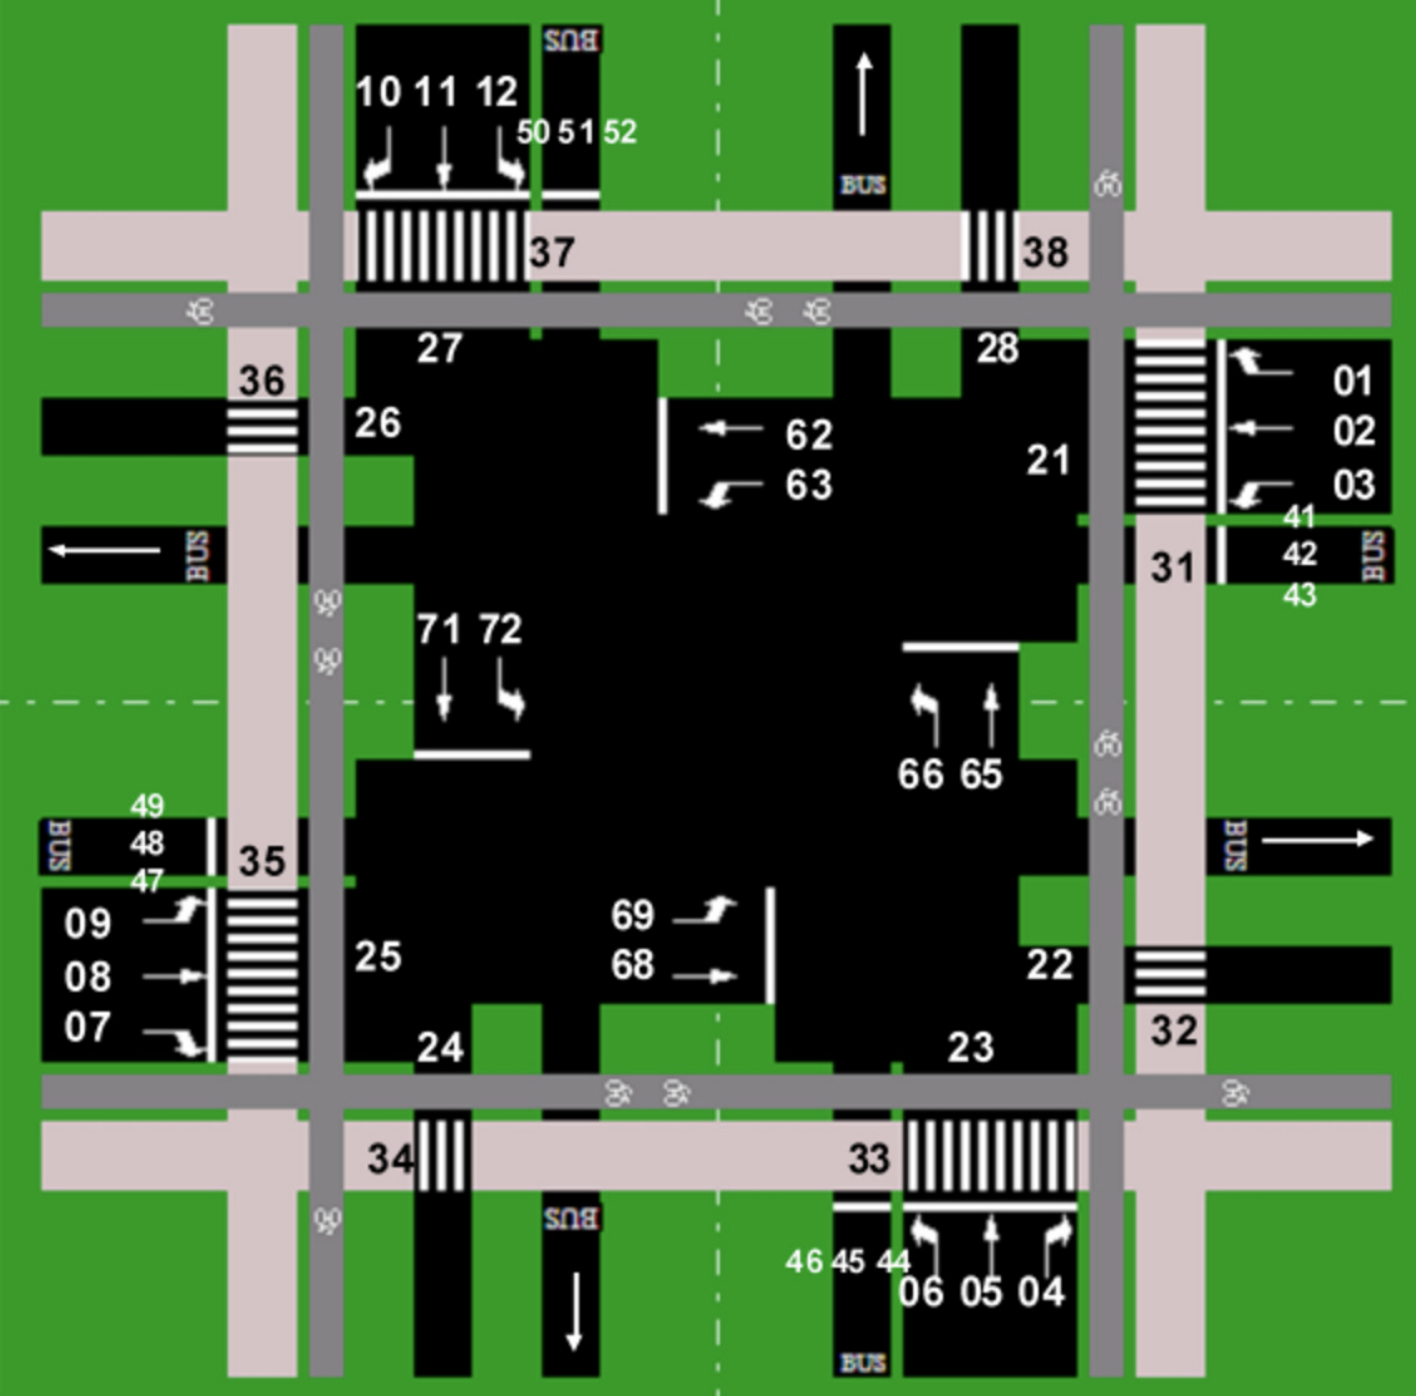
\includegraphics[width=8cm]{figures/standard.png}
    \caption{Cross Intersection layout}
    \label{fig: standard layout}
\end{figure}
  
\section{Research Questions}
To address the issue outlined in section \ref{section:Problem Statement}, this thesis presents a research objective that leads to the formulation of the research question.
\subsection{Research Objective}
The PF-SIQE, designed for real-time queue length estimation, is able to offer crucial inputs to real-time traffic signal controllers and serve as I2V (Infrastructure to Vehicle) information for connected vehicles. This could lead to improved performance at intersections, marked by reductions in traffic delays, vehicle emissions, and the incidence of vehicle crashes.
To achieve the development of the PF-SIQE, here are some specific research objectives:
\begin{enumerate}
  \item Develop a PF-SIQE architecture, along with the algorithm framework.
  \item Study various detection technologies, their outputs and the corresponding noise distribution.
  \item Building a modular mathematical model and implement in simulation.
  \item Validation of the PF-SIQE.
  \item Test the performance of the PF-SIQE to different factors such as the number of particles, penetration rate of the floating sensor, placement of loop detectors, probability of choosing stop within dilemma zone, initial condition, etc.
\end{enumerate}
\subsection{Research Contribution}
The primary contribution of this thesis is the development of a modular, scalable, flexible, and adaptable particle filter-based framework, specifically designed for real-time queue length estimation at signalized intersections. The framework is divided into three key modules: the state transition function module, the measurement function module, and the particle filter module. This modularity allows for the integration of various microscopic traffic flow models, as well as data from different detection technologies, such as loop detectors and floating car data, making the framework highly adaptable to diverse traffic conditions and data sources. 

A notable novelty of this work lies in its ability to handle uncertainties, including those with non-Gaussian noise distributions, which are common in real-world traffic scenarios. While the focus of this thesis is on signalized intersections, the framework itself has the potential to be extended to other types of intersections and roadway environments in future research. Further detailed contributions are discussed in Section \ref{LR: Conclusion}.

\subsection{Main Research Question}
How can a novel Particle Filter-based Signalized Intersection Queue Estimator (PF-SIQE) be developed for real-time queue length estimation using the particle filter algorithm, while accommodating different traffic flow models, detection technologies, and uncertainties?


\subsection{Sub Research Questions}
The sub-questions correspond directly to the research objectives:
\begin{enumerate}
  \item What is the PF-SIQE architecture along with particle filter algorithm framework? What are the modules of the framework?
  \item What are the common detection technologies? What are their output measurements and the corresponding noise characteristics?
  \item What are the mathematical descriptions of each modules in PF-SIQE framework?
  \item How to design the experiment scenarios in order to validate the PF-SIQE?
  \item What interested factors are selected to implement the sensitivity test? And why?
  \item How to abstract road layout features into the PF-SIQE architecture (future research recommendations)?
  %\item Study the estimation accuracy (also considering computational time, variance, etc.) considering (1) different penetration of probe vehicle or connected vehicle (ranging from 10\% to 90\% in increments of 10\%); (2) different numbers of loop detectors (increasing from 2 to 10); (3) the effective number of particle for various set-ups; (4) different update periods; (5) different data sources:  a. loop detector, b. probe vehicle or connected vehicle data, c. fusing loop detector and probe vehicle or connected vehicle data. (6) link length and vehicle length.
\end{enumerate}
\section{Research outline}
The research approach will result in an outline of the thesis. The list of contents at the chapter level is presented, describing the structure of the Thesis.
\begin{enumerate}
  \item Preface, Abstract, Nomenclature.
  \item Introduction, with the background and problem statement of the traffic problems, the corresponding research objectives, research questions and research contributions. 
  \item Literature review considering to:
  \begin{itemize}
      \item Comprehensive review of the real-time queue estimation methods at signalized intersection in terms of queue definition, time scale, algorithms and uncertainties.
      \item Comprehensive review of the detection technologies in terms of roadside sensors and floating sensors.
      \item Conclusion of the detailed contributions.
  \end{itemize}
  \item Methodology considering to:
  \begin{itemize}
      \item The PF-SIQE Architecture.
      \item Mathematical descriptions of the three modules: the state transition function module, the measurement function module, and the particle filter module.
  \end{itemize}
  \item Experimental simulation considering to:
  \begin{itemize}
      \item Validation of the PF-SIQE framework.
      \item Sensitivity tests to different factors such as the number of particles, penetration rate of the floating sensor, placement of loop detectors, probability of choosing stop within dilemma zone, initial condition, etc.
      \item Results and interpretation.
  \end{itemize}
  \item Discussion, conclusion, and recommendation considering to:
  \begin{itemize}
      \item Discussions on research findings, research questions, and methodology assumptions.
      \item Conclusions and implications.
      \item Recommendation for future works.
  \end{itemize}
  \item Bibliography and Appendices.
\end{enumerate}
Next chapter will present a very comprehensive literature review.